\documentclass[12pt,a4paper]{article}

\usepackage[utf8]{inputenc}
\usepackage{graphicx}
\usepackage{float}

\begin{document}

\title{MI-PAA 2015 4.ukol \\
}
\author{Tomas Nesrovnal\\nesrotom@fit.cvut.cz}
\date{\today}
\maketitle

\section{Zvolený algoritmus}
Simulovaná evoluce

\subsection{Jedinec}
Jedinec v populaci je jednorozmerne bitove pole, kdy jednotlivy bit znaci pritomnost predmetu v batohu.

\subsection{Fitness}
Zde jsem zvolil jednoduche a primocare reseni a to, ze fitness jedince je celkova cena. Pokud je prekrocena kapacita, je fitness 0.

Mozne vylepseni by bylo priradit kladnou fitness i nevalidnim resenim, ale s dobrym potencialem.

\subsection{Inicializace}
Kazdy jedinec je nahodne generovan (kazdy bit ma 50 \% sanci byt 1) do te doby, dokud nebude mit $fitness > 0$.

\subsection{Crossover}
Jednobodove a dvoubodove krizeni.

\subsection{Mutace}
Pri mutaci je s jistou (velmi malou) pravdepodobnosti zmutovan kazdy jedinec.

\subsection{Selekce}
Turnajova selekce.

\subsection{Vliv nahody}
Pred kazdym merenim byla vyresetovana nahoda. Protoze je implementace v C, vola se srand(0).


\section{Mereni}

\subsection{Metoda}

Mereni jsem provedl na setu vygenerovanem pomoci generatoru:

\texttt{.\/knapgen -I 42 -n 300 -N 1 -m 0.5 -k 0.5 -W 1000 -C 1000 -d 0}

\subsection{Spravnost vysledku}
Spravnost vysledku byla overena porovnanim vysledku s vysledkem metody dynamickeho programovani. Je jasne, ze pro velke sety nejsou vysledky ty uplne nejlepsi, pro mensi sety s dobrym nastavenim byly nalezeny optimalni reseni.

\subsection{Na cem bylo mereno}
Intel(R) Core(TM) i3-2328M Processor (3M Cache, 2.20 GHz), gcc 4.9.2 (-Ofast), OS GNU/Linux Lubuntu 14.04 64bit

\subsection{Mutace}

Vyvoj mutace v 0.1 \%.
Nastaveni: opakovani 1000, populace 1000, velikost turnaje 50

\begin{figure}[H]
	\caption{Vliv mutace}
 	\centerline{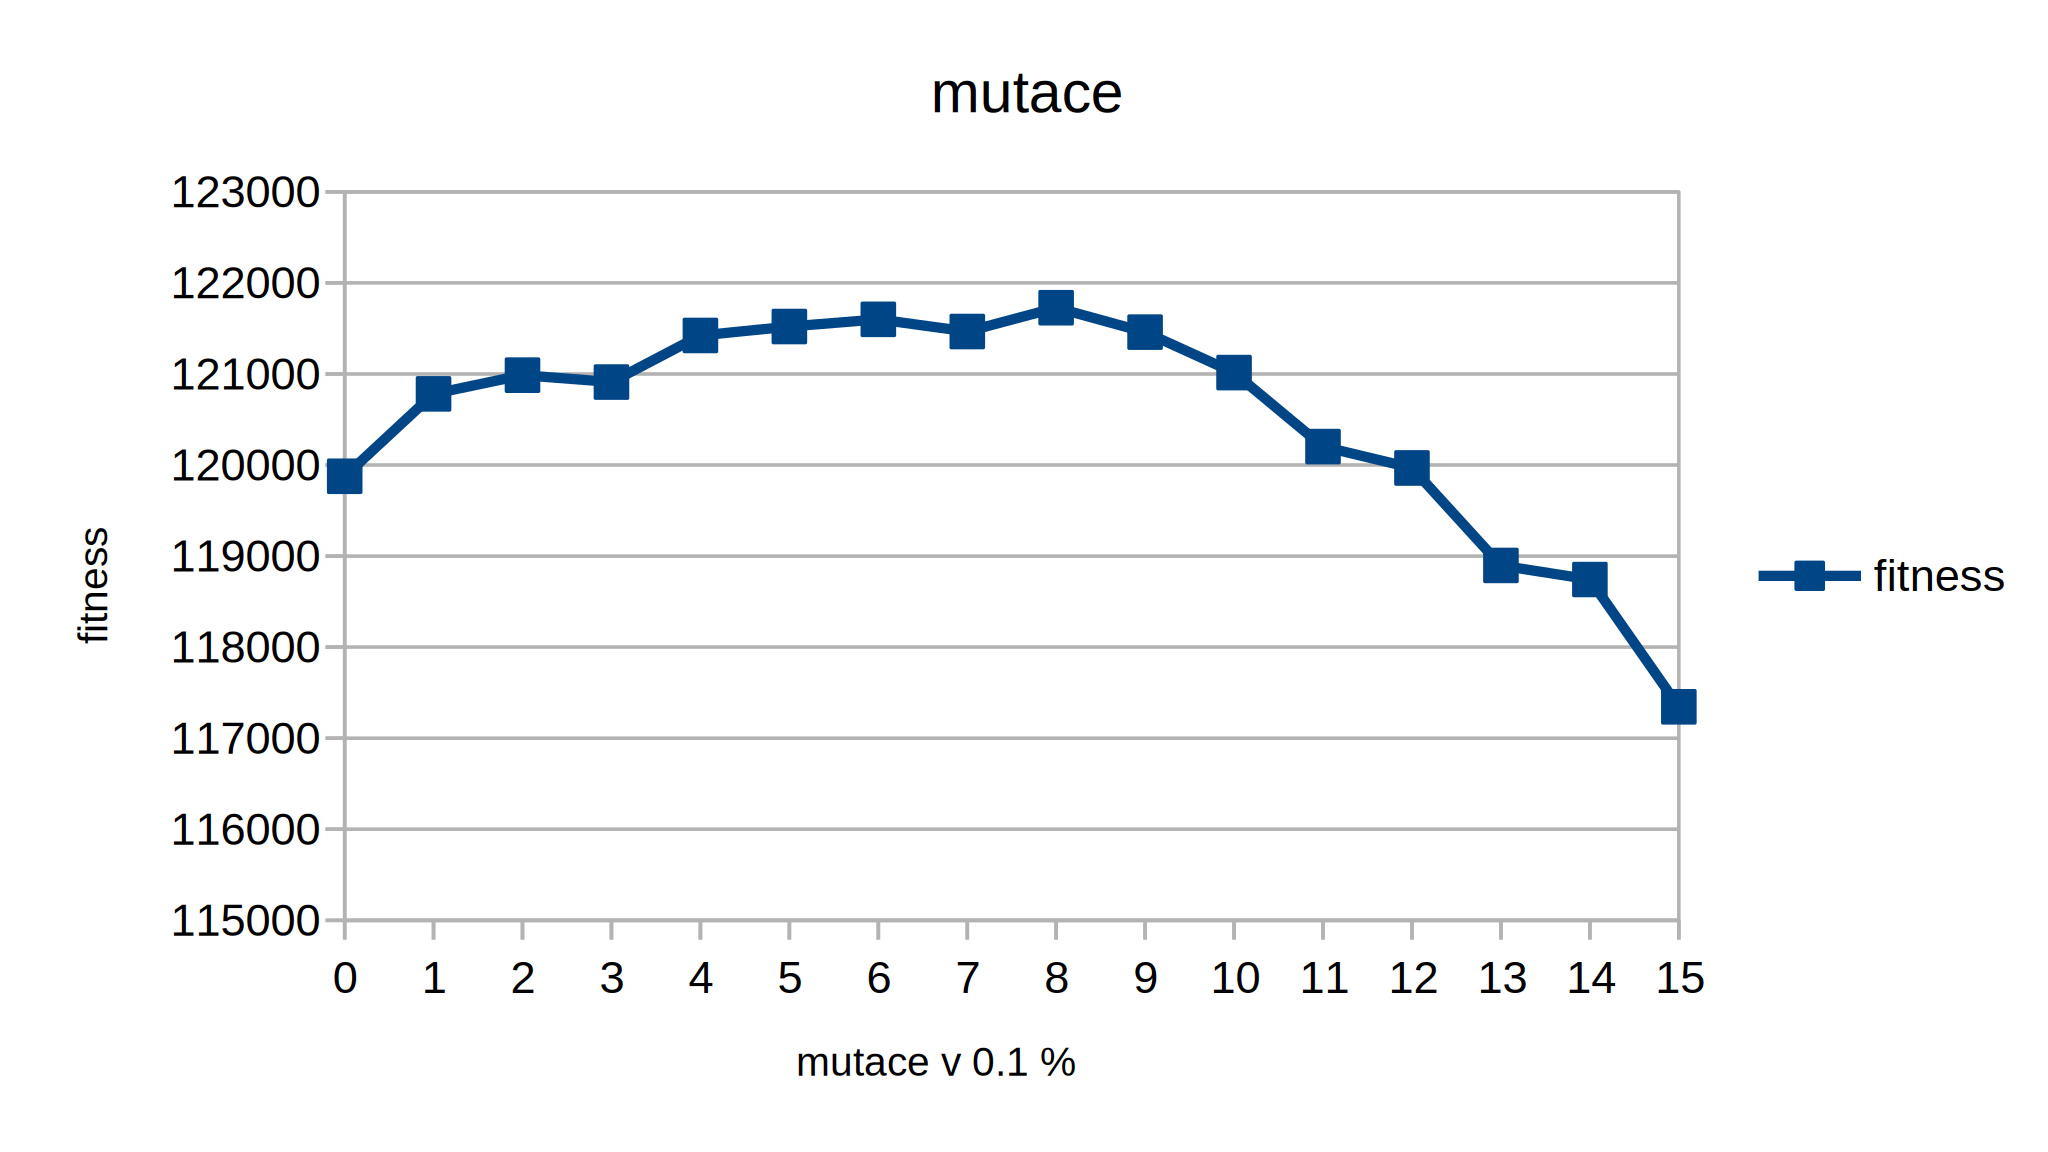
\includegraphics{mutation.pdf}}
\end{figure}

\subsection{Velikost turnaje}
Nastaveni: opakovani 1000, populace 1000, pravdepodobnost mutace jedince 0.8 \%
\begin{figure}[H]
	\caption{Vliv velikosti tournamentu}
 	\centerline{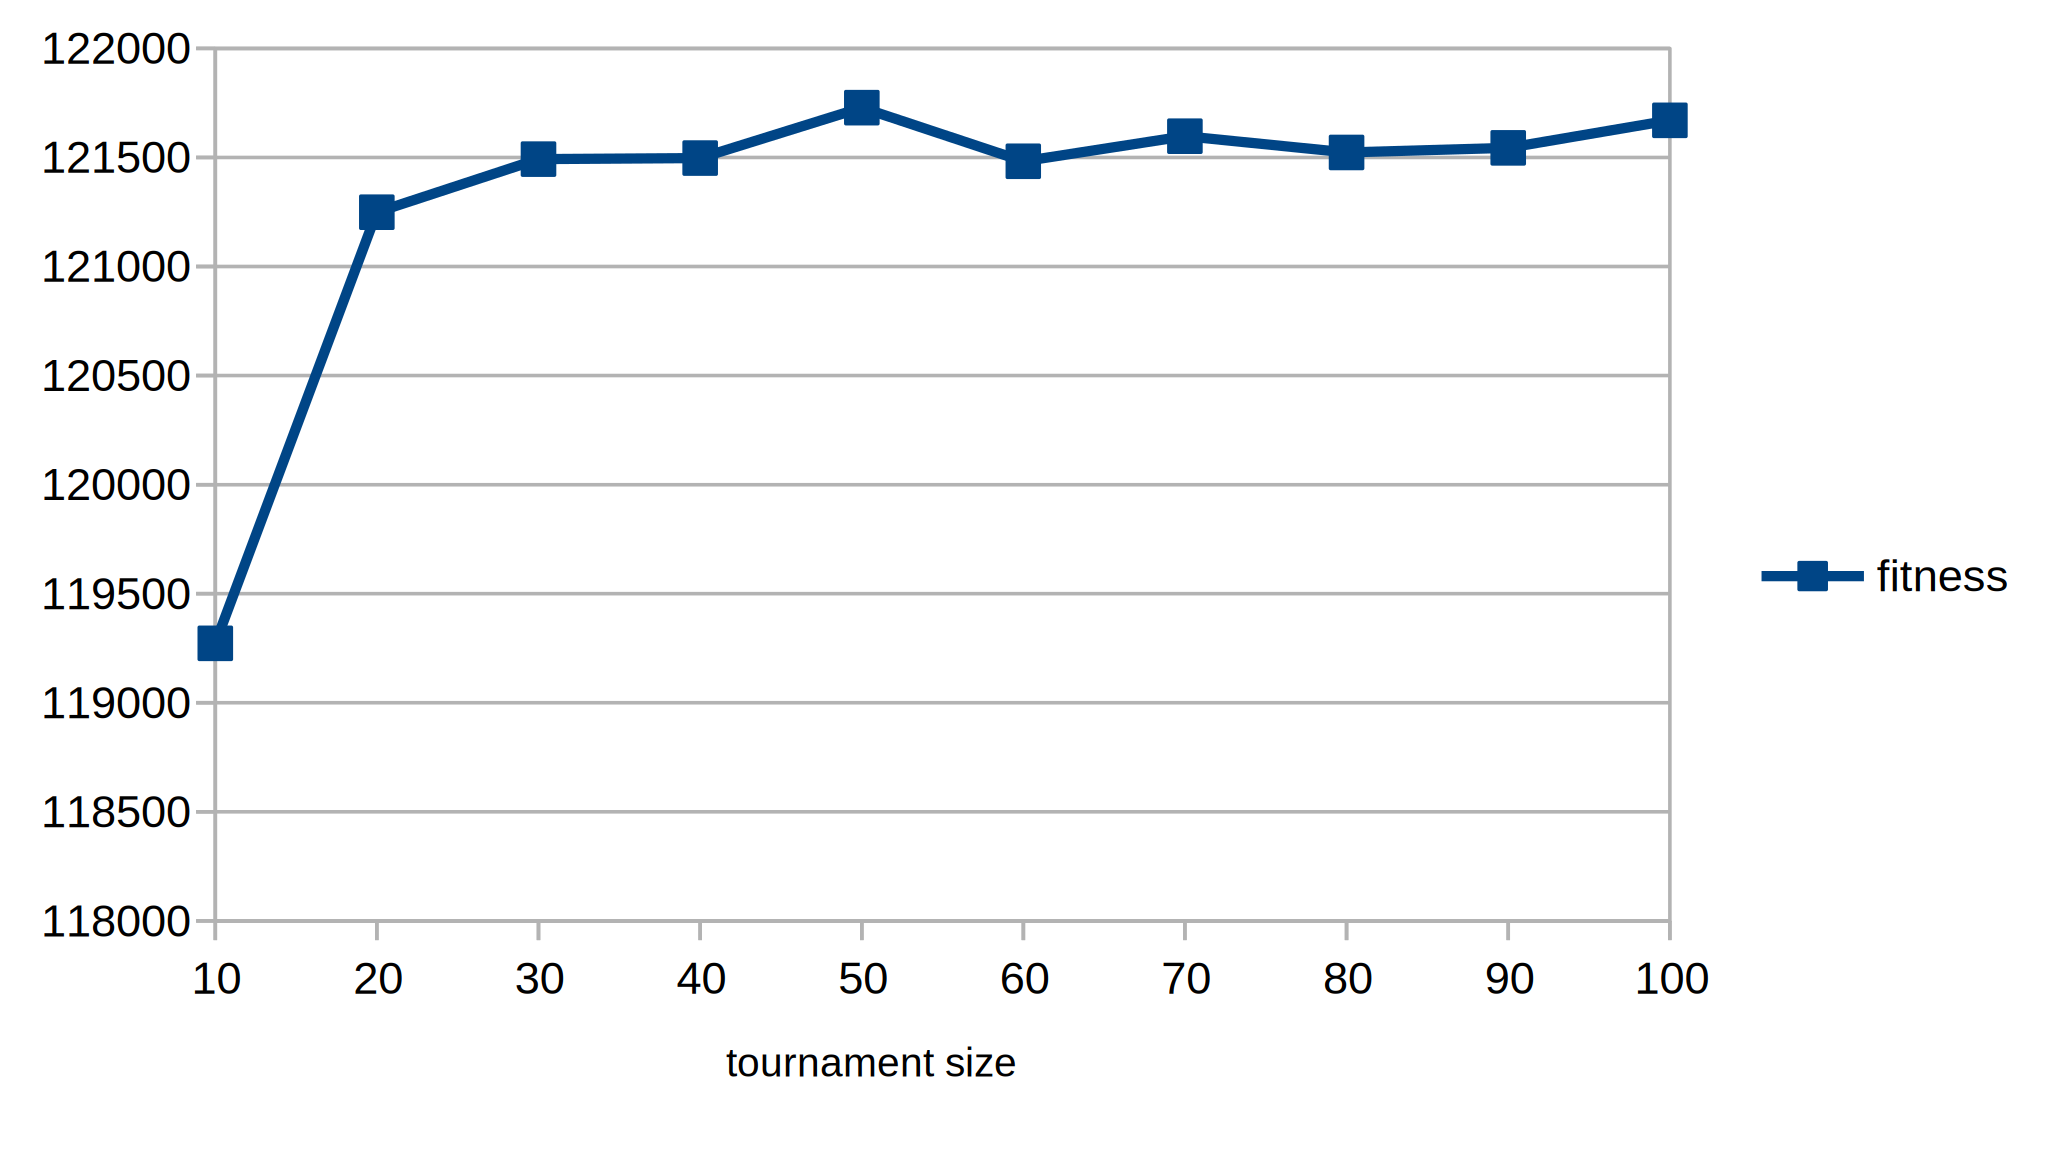
\includegraphics{tournament.pdf}}
\end{figure}

\subsection{Krizeni}

Pomoci jednobodoveho krizeni bylo dosazeno vysledku 121365. Pomoci dvoubodoveho 121728.

\subsection{Porovnani s dynamickym programovanim: cas a vysledek}
Dynamicke programovani za 0.079516 sekundy spocitalo vysledek 121794.
Simulovana evoluce za 6.359731 sekund spocitala vysledek 121728.

Nutno podotknout, ze slozitost simulovane evoluce zavisi na parametrech, hlavne je to pocet opakovani, velikost populace a v male mire zalezi i na velikosti turnaje.

\section{Zaver}

Simulovana evoluce ma vyhodu v tom, ze po tom co zakodujeme jedice do genomu a vytvorime fitness funkci, udela zbytek prace za nas.

%%%%%%%%%%%%%%%%%%%%%%%%%%%%%%%%%%%%%%%%%%%%%%%%%%%%%%%%%%%%%%%%%%%%%%%%%%%%%%
\end{document}
